\documentclass[11pt]{article}
\usepackage{amsmath,amssymb,amsthm}
\usepackage{booktabs}
\usepackage{natbib}
\usepackage{tikz}
\usetikzlibrary{arrows.meta, positioning, calc}
\usepackage[margin=1in]{geometry}
\usepackage{xcolor}
\usepackage{graphicx}
\usepackage{siunitx}

% \newcommand{\new}[1]{{\color{blue}#1}}
% \newcommand{\edit}[1]{{\color{magenta}#1}}
\newcommand{\new}[1]{#1}
\newcommand{\edit}[1]{#1}

\definecolor{darkgreen}{RGB}{0,100,0}

\newcommand{\E}{\mathbb{E}}
\newcommand{\Var}{\mathrm{Var}}
\newcommand{\ind}{\mathbf{1}}

\title{Supplementary Information:\\Maximum Likelihood Estimation of Intermittent Methane Emissions}
\author{}
\date{}

\begin{document}
\maketitle

\tableofcontents
\newpage

%==============================================================================
% [PB — new SI section: correlated-mean derivation, pulled out of the intro]
\section{Cost of Ignoring Correlation}
\label{sec:corr_mean_SI}
%==============================================================================

\new{This section formalises the claim made in Section~1 of the main text that treating positively-correlated observations as independent inflates estimator variance beyond what sample size alone implies. The argument is a standard result on the variance of linear estimators of a common mean, reproduced here to clarify its connection to the variance gains obtained by the MLE.}

\new{Consider a vector of samples $\mathbf{x} = (x_1, \ldots, x_N)^\top$ with common mean $\mathbb{E}[x_i] = \mu$ and covariance matrix $\mathbf{C} = \mathrm{Cov}(\mathbf{x})$. Writing $\mathbf{1}$ for the $N$-vector of ones, the empirical mean can be expressed as $\bar x = N^{-1} \mathbf{1}^\top \mathbf{x}$, with variance
\begin{equation}
    \Var(\bar x) = \frac{1}{N^2} \mathbf{1}^\top \mathbf{C}\, \mathbf{1}.
\end{equation}
When $\mathbf{C} = \sigma^2 \mathbf{I}$ this reduces to the familiar $\sigma^2/N$. For general $\mathbf{C}$ with positive off-diagonal entries, $\mathbf{1}^\top \mathbf{C}\, \mathbf{1} > N \sigma^2$, so $\Var(\bar x)$ exceeds $\sigma^2/N$ by an amount that grows with the off-diagonal mass of $\mathbf{C}$.}

\new{Among all linear unbiased estimators of $\mu$ — that is, all estimators of the form $\mathbf{w}^\top \mathbf{x}$ with $\mathbf{w}^\top \mathbf{1} = 1$ — the one with minimum variance is the inverse-covariance-weighted mean
\begin{equation}
    \hat\mu_\star 
    = \frac{\mathbf{1}^\top \mathbf{C}^{-1} \mathbf{x}}{\mathbf{1}^\top \mathbf{C}^{-1} \mathbf{1}},
    \qquad
    \Var(\hat\mu_\star) = \frac{1}{\mathbf{1}^\top \mathbf{C}^{-1} \mathbf{1}}.
    \label{eq:gls_SI}
\end{equation}
This follows from Lagrangian minimisation of $\mathbf{w}^\top \mathbf{C}\, \mathbf{w}$ subject to $\mathbf{w}^\top \mathbf{1} = 1$. The empirical mean achieves this minimum only when $\mathbf{C} \propto \mathbf{I}$; otherwise it is strictly sub-optimal, and the gap $\Var(\bar x) - \Var(\hat\mu_\star)$ measures the information that the empirical mean discards by treating the samples as exchangeable.}

\new{As a simple illustration, consider the compound-symmetry structure in which $\mathbf{C}$ has equal diagonal entries $\sigma^2$ and equal off-diagonal entries $\rho \sigma^2$. Then
\begin{equation}
    \Var(\bar x) = \frac{\sigma^2}{N}\bigl[1 + (N-1)\rho\bigr],
\end{equation}
so that doubling $N$ does not halve the variance when $\rho > 0$: the benefit of additional samples is attenuated by the correlation. In the limit $\rho \to 1$, $\Var(\bar x) \to \sigma^2$ regardless of $N$, since the $N$ samples carry the information of a single draw.}

\new{In the methane-monitoring context, the correlation structure is richer than compound symmetry: samples within a single emission event are highly correlated, while samples across distinct events are approximately independent. The effective correlation $\bar\rho$ therefore depends on the fraction of revisits that fall within the same event, which in turn depends on the emission-duration distribution and the sampling cadence. The POD-weighted estimator of Section~3.1.3 of the main text is essentially an empirical mean over weighted detections and so inherits the variance inflation described above. By contrast, the MLE models the latent state sequence explicitly: events are identified as such, within-event observations are combined into a single estimated emission size, and the resulting per-event sample behaves more like an independent draw from the emission distribution. This is the mechanism by which the MLE recovers (in part) the information that the empirical mean discards.}

%==============================================================================
\section{Model Structure}
\label{sec:model}
%==============================================================================

We model methane emissions and their observation as a four-layer hierarchical process. The first two layers describe the latent emission process; the second two describe how emissions are observed. Figure~\ref{fig:model} illustrates the dependencies.

\begin{figure}[h]
\centering
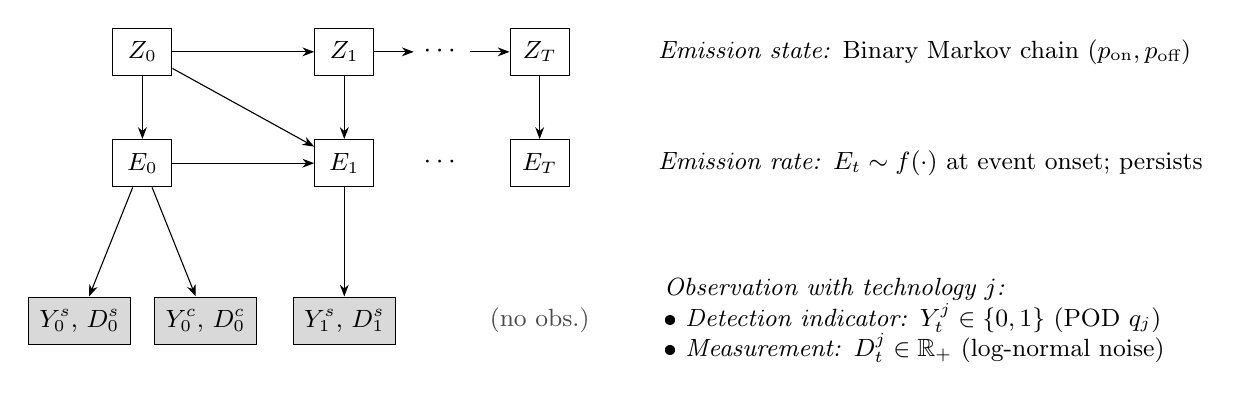
\begin{tikzpicture}[
    node distance=0.8cm and 1.8cm,
    box/.style={draw, minimum width=0.75cm, minimum height=0.6cm, font=\small},
    obs/.style={box, fill=gray!30},
    obswide/.style={draw, fill=gray!30, minimum width=1.3cm, minimum height=0.6cm, font=\small},
    arrow/.style={-{Stealth[length=1.5mm]}},
]
% Layer 1: Emission state
\node[box] (Z0) {$Z_0$};
\node[box, right=of Z0] (Z1) {$Z_1$};
\node[right=0.5cm of Z1] (Zdots) {$\cdots$};
\node[box, right=0.5cm of Zdots] (ZT) {$Z_T$};
\draw[arrow] (Z0) -- (Z1);
\draw[arrow] (Z1) -- (Zdots);
\draw[arrow] (Zdots) -- (ZT);

% Layer 2: Emission rate
\node[box, below=of Z0] (E0) {$E_0$};
\node[box, below=of Z1] (E1) {$E_1$};
\node (Edots) at ([yshift=-1.4cm] Zdots) {$\cdots$};
\node[box, below=of ZT] (ET) {$E_T$};
\draw[arrow] (Z0) -- (E0);
\draw[arrow] (Z1) -- (E1);
\draw[arrow] (ZT) -- (ET);
\draw[arrow] (E0) -- (E1);
\draw[arrow] (Z0) -- (E1);

% Layer 3: Detection + measurement
\node[obswide] (O0s) at ([xshift=-0.8cm, yshift=-2.0cm] E0) {$Y_0^s,\, D_0^s$};
\node[obswide] (O0c) at ([xshift=+0.8cm, yshift=-2.0cm] E0) {$Y_0^c,\, D_0^c$};
\draw[arrow] (E0) -- (O0s);
\draw[arrow] (E0) -- (O0c);

\node[obswide] (O1s) at ([xshift=0cm, yshift=-2.0cm] E1) {$Y_1^s,\, D_1^s$};
\draw[arrow] (E1) -- (O1s);

\node[font=\small, text=gray!60!black] (noobs) at ([yshift=-2.0cm] ET) {(no obs.)};

% Right-side annotations
\node[right=1.0cm of ZT, font=\small, align=left] {%
    \textit{Emission state:} Binary Markov chain $(p_{\text{on}}, p_{\text{off}})$};
\node[right=1.0cm of ET, font=\small, align=left] {%
    \textit{Emission rate:} $E_t \sim f(\cdot)$ at event onset; persists};
\node[right=0.7cm of noobs, font=\small, align=left] {%
    \textit{Observation with technology $j$:}\\
    \textbullet~\textit{Detection indicator:} $Y_t^j\in\{0,1\}$ (POD $q_j$)\\
    \textbullet~\textit{Measurement:}
    $D_t^j\in\mathbb{R}_+$ (log-normal noise)};

\end{tikzpicture}
\caption{Graphical model for intermittent emissions with imperfect detection. Shaded nodes are observed; unshaded nodes are latent. The emission state $Z_t$ follows a two-state Markov chain. The emission rate $E_t$ is drawn at event onset and persists until the event ends. At each time step, the true rate may produce zero, one, or two pairs of detection/measurement outcomes depending on which technologies are deployed: $Y_t^j$ (detection indicator) and $D_t^j$ (measured value) for technology $j \in \{s, c\}$. Here $t = 0$ illustrates a dual-observation time step, $t = 1$ a single-technology observation, and $t = T$ an unobserved time step. When both technologies are present their detections are conditionally independent given $E_t$.}
\label{fig:model}
\end{figure}

\paragraph{Emission state.} The binary state $Z_t \in \{0,1\}$ indicates whether the source is emitting at time $t$. It evolves as a Markov chain with transition probabilities $p_{\text{on}} = P(Z_t = 1 \mid Z_{t-1} = 0)$ and $p_{\text{off}} = P(Z_t = 0 \mid Z_{t-1} = 1)$. The transition matrix is
\begin{equation}
    \mathbf{T} = \begin{pmatrix} 1 - p_{\text{on}} & p_{\text{on}} \\ p_{\text{off}} & 1 - p_{\text{off}} \end{pmatrix},
\end{equation}
with stationary distribution $\pi_{\text{on}} = p_{\text{on}}/(p_{\text{on}} + p_{\text{off}})$ and $\pi_{\text{off}} = p_{\text{off}}/(p_{\text{on}} + p_{\text{off}})$. The mean emission duration is $\tau = 1/p_{\text{off}}$ time steps.

In oil and gas contexts, $p_{\text{on}}$ reflects how frequently new emission events begin: equipment failures, valve malfunctions, or intentional venting operations. A value of $p_{\text{on}} = 0.1$ means that on any given \edit{hour} when the source is inactive, there is a 10\% chance a new emission begins within one time step. The parameter $p_{\text{off}}$ reflects how quickly emissions resolve, either through repair or self-resolution. A value of $p_{\text{off}} = 0.05$ implies emissions last on average $\tau = 20$ hours.

\paragraph{Emission rate.} When $Z_t = 1$, the source emits at rate $E_t > 0$; when $Z_t = 0$, we define $E_t = 0$. The emission rate evolves according to
\begin{equation}
    E_t \mid Z_t, Z_{t-1}, E_{t-1} = 
    \begin{cases}
        0 & \text{if } Z_t = 0 \\
        E_{t-1} & \text{if } Z_t = 1 \text{ and } Z_{t-1} = 1 \\
        \sim f(\cdot) & \text{if } Z_t = 1 \text{ and } Z_{t-1} = 0
    \end{cases}
\end{equation}
That is, a new rate is drawn from a distribution $f(\cdot)$ whenever an emission event begins, and the rate persists until the event ends. This reflects the physics of equipment malfunctions, which typically emit at a characteristic rate determined by the failure mode until it stops.

\paragraph{Choice of emission-rate distribution.}
We model $f$ as log-normal: $\log E \sim \mathcal{N}(\mu_{\log}, \sigma_{\log}^2)$ given a new emission event. This is consistent with the heavy-tailed distributions observed empirically for oil and gas emissions~\citep{Brandt2016, ZavalaAraiza2015}, where a small fraction of sources accounts for the majority of total emissions. With $\mu_{\log} = 3.787$ and $\sigma_{\log} = 0.5$ (the baseline configuration used in the simulations), the median emission rate is approximately $44$~kg/h with overall mean $50$~kg/h, and the distribution spans roughly $23$ to $84$~kg/h between the 10th and 90th percentiles. In the single-site interpretation, this means that successive emission events at a given facility vary substantially in magnitude: most events are moderate, but occasional large releases occur with non-negligible probability. The log-normal form captures this right-skewed, positive-support behavior while remaining analytically tractable. Importantly, however, the estimation procedure itself is largely agnostic to the parametric form of $f$. In the IPW correction (Step~2), the reweighting is computed from the empirical distribution of detected emission rates and the detection-probability curve, without assuming a parametric form. The forward algorithm (Step~3) depends on $f$ only through the scalar $\kappa$, which can itself be estimated empirically. We use the log-normal in our simulations to generate synthetic data and to verify the method, but alternative specifications, including heavy-tailed or nonparametric forms, can be accommodated without modifying the algorithm.

An important distinction arises between the distribution of emission rates \emph{across sites} and the distribution of emission rates \emph{at a single site over time}. Much of the literature on heavy-tailed methane emissions concerns the cross-site distribution: \citet{Sherwin2024Nature} show that site-level emission rates across a basin exhibit roughly log-normal behavior at small sizes but transition to approximate power-law behavior above 10 to 100~kg/h, with a log-normal fit underestimating or overestimating basin-level mean emissions by up to 58 to 170\% depending on the region. However, this cross-site heterogeneity reflects differences in equipment types, operational practices, and geology across facilities. Our distribution $f$ describes a different object: the rates of successive emission events at a \emph{single} facility, which are driven by the specific failure modes present at that site and are likely to exhibit less extreme tail behavior. The heavy-tailed cross-site distribution emerges not from $f$ itself but from the variation in facility-level estimates $\hat{\mu}$ when aggregated across sites. Indeed, a mixture of site-specific log-normals with different means can produce power-law-like tails at the population level, even if no individual site has a power-law distribution.

This distinction relates to the question of ergodicity in basin-scale estimation. Some approaches treat a single comprehensive snapshot across many sites as equivalent to repeated observations of one site over time, assuming that the cross-sectional distribution equals the temporal distribution. \citet{Chen2022EST} address this carefully in their basin-wide aerial survey of the New Mexico Permian: they show that summing persistence-weighted, source-level averages over a near-complete census ($>$90\% of assets) yields an unbiased estimate of basin-total emissions under three conditions: (i) coverage decisions are independent of emission status, (ii) sampled assets are representative of the population, and (iii) the emission distribution is stationary over time. Crucially, this argument does not require that all sites share the same emission parameters. It is an unbiased-sampling result, not an ergodic equivalence between time and ensemble averages. The authors acknowledge that for any single intermittent source, a small number of observations cannot fully characterize its temporal variation.

Our framework addresses this limitation and operates at whatever level of aggregation the analyst specifies. Given a collection of observations, whether from a single site over time, a group of operationally similar facilities, or an entire sub-basin, the self-consistent loop jointly corrects for intermittency and detection bias under the assumed emission and measurement model. The only structural requirement is that the pooled observations plausibly share the emission and activity parameters. Although we use a single-source, two-state Markov chain for intermittency in this paper, the framework accommodates richer latent-state models without modifying the overall algorithmic structure. For instance, a site with multiple independent emission sources (e.g., a well pad with both a compressor and a tank battery) could be modeled with a multi-source Markov chain, where each component has its own on/off dynamics and the observed site-level emission is the superposition. Similarly, semi-Markov processes with duration-dependent transition probabilities or multi-state models distinguishing between different emission regimes could be substituted. In the single-site case with dense temporal coverage, the estimate $\hat{\mu}_i$ converges to the true time-averaged rate; when observations are sparse, the parametric model provides regularization that a simple detection-to-overflight ratio cannot. Basin-level estimation then proceeds by aggregating estimates across groups, without requiring that all sites in the basin share the same parameters.

\paragraph{Measurement process.} The two monitoring technologies have different deployment physics. At each time step $t$, a snapshot observation occurs independently with probability $p_{\text{snap}}$. Continuous monitors follow a renewal process: at each unmonitored step, a Bernoulli draw with probability $p_{\text{cont}}$ triggers deployment of a monitor that runs for $T_{\text{cont}}$ contiguous steps; during an active window no new draw is made. Let $\mathcal{J}_t \subseteq \{\text{snap}, \text{cont}\}$ denote the set of active technologies at time $t$; a given time step may have $|\mathcal{J}_t| = 0, 1,$ or $2$.

Detection probability depends on the emission rate through a probability-of-detection (POD) curve:
\begin{equation}
    q_j(e)
    \doteq p(Y^j_t=1\mid Z_t=1,E_t=e) 
    = \frac{1}{1+(\theta_j/e)^k_j},
\end{equation}
where $\theta_j$ is the 50\% detection threshold and $k_j$ controls the steepness of the transition from non-detection to reliable detection.

If detected, the measured rate $D_t$ differs from the true rate due to quantification uncertainty:
\begin{equation}
    D_t = E_t \cdot \exp(\varepsilon_t), \quad \varepsilon_t \sim \mathcal{N}(-\sigma^2/2, \sigma^2)
\end{equation}
where $\sigma_j$ depends on the technology ($\sigma_{\text{snap}} = 0.05$, $\sigma_{\text{cont}} = 0.2$ in the baseline).

\paragraph{Target estimand.} Our goal is to estimate the time-averaged emission rate:
\begin{equation}
    \mu = \E[E_t] = \pi_{\text{on}} \cdot \E[E_t \mid Z_t = 1] = \pi_{\text{on}} \cdot \mu_{\text{emit}}.
\end{equation}

\paragraph{Special cases.}
When $p_{\text{cont}} = 0$, no continuous monitoring windows are triggered and the model reduces to snapshot-only observation at rate $p_{\text{snap}}$. When $p_{\text{snap}} = 0$, only continuous observations contribute data. Setting $p_{\text{snap}} = 1$ and $p_{\text{cont}} = 0$ recovers the single-technology model where every time step is observed by the snapshot sensor.

%==============================================================================
\section{The Inference Challenge}
\label{sec:challenge}
%==============================================================================

To understand why inference is difficult, it helps to consider progressively more realistic versions of the problem.

\subsection{Case 1: Perfect detection without emission rates}

Consider first the simplest setting: we observe the emission state directly ($Y_t = Z_t$) and ignore emission rates entirely. With observations at times $t_1, \ldots, t_N$ (not necessarily consecutive), the likelihood is
\begin{equation}
    \mathcal{L}(p_{\text{on}}, p_{\text{off}}) = \pi_{Z_{t_1}} \prod_{k=1}^{N-1} [\mathbf{T}^{\Delta_k}]_{Z_{t_k}, Z_{t_{k+1}}},
\end{equation}
where $\Delta_k = t_{k+1} - t_k$ is the gap between observations and $\mathbf{T}^{\Delta}$ is the $\Delta$-step transition matrix and $\pi=(\pi_\text{off}, \pi_\text{on})^T$. We can count transitions directly and the problem is entirely tractable.

\subsection{Case 2: Perfect detection with emission rates}

Now suppose we observe both the emission state and the emission rate (with measurement noise). Because we observe the states directly, we can identify exactly which time steps belong to which emission events. Consecutive ON states with no intervening OFF state share the same underlying rate; an ON state following an OFF state begins a new event with a fresh draw from $f$. The likelihood can be written down explicitly and maximized jointly over all parameters. No marginalization over latent variables is required.

\subsection{Case 3: Imperfect detection}

Now we confront the realistic setting: detection depends on emission rate, so large emissions are detected reliably while small emissions may be missed. A non-detection ($Y_t = 0$) is ambiguous: it could mean the source was OFF ($Z_t = 0$), or that the source was ON but the emission was too small to detect ($Z_t = 1$ with small $E_t$). The likelihood must marginalize over both the unobserved states and the unobserved emission rates:
\begin{equation}
    \mathcal{L} = \sum_{\mathbf{Z}} \int P(\mathbf{Z}) \, P(\mathbf{E} \mid \mathbf{Z}) \, P(\mathbf{Y} \mid \mathbf{Z}, \mathbf{E}) \, P(\mathbf{D} \mid \mathbf{E}, \mathbf{Y}) \, d\mathbf{E}.
    \label{eq:full_likelihood_SI}
\end{equation}

This high-dimensional integral has no closed form because the continuous emission rates $E_t$ appear nonlinearly inside the POD function $q(E_t)$. Moreover, rate persistence within emission events couples the integrands across time steps. Direct maximization is therefore intractable.

\subsection{A tractable relaxation}

The key insight enabling our approach is that we can work with the \emph{marginalized detection probability}:
\begin{equation}
    \kappa_j
    \doteq p(Y_{t}^j=1\mid Z_t=1)
    = \int q_j(e)\,f(e)\,\mathrm{d}e
    =\E[q_j(E_t) \mid Z_t = 1].
\end{equation}

If we treat $\kappa$ as known, the observation model simplifies dramatically: this is a standard two-state HMM with known emission probabilities, and the likelihood can be computed in $O(N)$ time using the forward algorithm (see Section~\ref{sec:forward}).

The remaining difficulty is that $\kappa$ depends on $f$, which we must estimate from the size-biased sample of detected emissions. Our algorithm addresses this through iteration: we alternate between estimating $f$ (correcting for detection bias given current state estimates) and estimating the transition probabilities (using the current estimate of $\kappa$).

%==============================================================================
\section{Alternative Estimation Approaches}
\label{sec:alternatives}
%==============================================================================

Before developing our approach, we considered several standard methods for hidden Markov model inference.

\subsection{Standard Baum--Welch algorithm}

The Baum--Welch algorithm is the canonical method for parameter estimation in hidden Markov models. To apply it here, one could discretize the emission-rate distribution into $K$ bins and define an HMM with $K+1$ states: one OFF state and $K$ ON states corresponding to different emission-rate ranges.

This approach has two fundamental limitations. First, standard Baum--Welch assumes observations at regular time intervals. Methane monitoring data are inherently irregular: satellites have revisit times of days to weeks; aircraft campaigns occur sporadically; continuous monitors have maintenance gaps. While one can interpolate the transition matrix or treat gaps as missing data, these workarounds introduce approximation errors.

Second, the M-step yields unconstrained probabilities for each emission-rate bin. There is no guarantee that the resulting distribution corresponds to a parametric family (e.g., log-normal) or even forms a smooth distribution. This is problematic because parametric structure enables extrapolation to emission rates below detection thresholds, which is critical since a significant fraction of total emissions may come from undetectable sources.

\subsection{Baum--Welch with parametric projection}

A natural modification is to run Baum--Welch and then project the resulting bin probabilities onto a parametric family. This preserves some structure but introduces approximation error: the projected distribution is not the true maximum likelihood estimate, and the two-stage procedure lacks theoretical guarantees on convergence or consistency.

\subsection{Continuous-time Markov chain formulation}

Formulating the emission process as a continuous-time Markov chain handles irregular gaps naturally: the transition matrix over any interval $\Delta$ is $\exp(\mathbf{Q}\Delta)$. However, exact inference requires numerical integration over emission rates at each observation time---computationally expensive when rates span several orders of magnitude. The resulting cost is prohibitive for applications involving hundreds to thousands of facilities.

\subsection{Comparison}

Table~\ref{tab:comparison} summarizes the tradeoffs. Our self-consistent loop combines the strengths of each while avoiding their limitations.

\begin{table}[h]
\centering
\caption{Comparison of estimation approaches for intermittent methane emissions with imperfect detection.}
\label{tab:comparison}
\begin{tabular}{lccccc}
\toprule
Method & \shortstack{Irregular\\gaps} & \shortstack{Non-\\detections} & \shortstack{Parametric\\structure} & \shortstack{Comput.\\cost} & \shortstack{Interpret-\\ability} \\
\midrule
Baum--Welch (discretized) & $\times^a$ & \checkmark & $\times$ & Low & Medium \\
Baum--Welch + projection & $\times^a$ & \checkmark & $\triangle^b$ & Medium & Medium \\
Continuous-time MC & \checkmark & \checkmark & \checkmark & High & High \\
Self-consistent loop & \checkmark & \checkmark & \checkmark & Medium & High \\
\bottomrule
\end{tabular}
\vspace{0.5em}
{\footnotesize $^a$Requires interpolation or missing-data treatment for gaps. $^b$Parametric form imposed by projection, not by MLE.}
\end{table}

%==============================================================================
\section{The Self-Consistent Loop Algorithm}
\label{sec:algorithm}
%==============================================================================

\subsection{Step 1: Event identification}

Consecutive detections may represent the same emission event observed multiple times, or distinct events separated by a period of inactivity. Distinguishing these cases matters: treating repeated observations of the same emission as independent will yield an under-estimated $\pi_\text{on}$; incorrectly merging distinct events over-estimates it.

We use a Bayesian linking model that combines temporal proximity with measurement similarity. For detections at times $t_i$ and $t_{i+1}$ with measurements $D_i$ and $D_{i+1}$, we compute the posterior probability that they belong to the same event:
\begin{equation}
    P(\text{same} \mid D_i, D_{i+1}, \Delta t) = \frac{P_{\text{prior}} \cdot \text{BF}}{1 + P_{\text{prior}} \cdot \text{BF}}.
\end{equation}

The temporal prior $P_{\text{prior}} = \exp(-\Delta t \cdot p_{\text{off}})$ reflects the probability that an emission persists over the gap $\Delta t = t_{i+1} - t_i$.

The Bayes factor (BF) compares two hypotheses: $H_{\text{same}}$, that both measurements come from the same underlying rate, versus $H_{\text{diff}}$, that they come from independent draws. Its derivation is given in Section~\ref{sec:bayes_factor}. We merge detections when $P(\text{same}) > 0.5$, proceeding sequentially through the detection sequence. For each identified event, we estimate the emission rate as the mean of its constituent measurements.

\paragraph{Multi-technology plume identification.}
When both technologies observe at the same time step and both produce a detection, these detections are always assigned to the same plume (same emission event). Their measurements are combined via inverse-variance weighted average in log-space \emph{before} computing the Bayes factor for linking with adjacent time steps. For detections at different time steps, the standard Bayesian linking procedure applies using the combined measurements and effective noise.



\subsection{Step 2: Emission-rate distribution}

The identified plumes provide a sample of emission rates biased toward large values. We correct for this using inverse-probability weighting (IPW). Each plume with estimated rate $\hat{e}_m$ receives weight $w_m = 1/P_{\text{det}}(\hat{e}_m)$, where $P_{\text{det}}(e)$ is the marginal probability that an emission event of size~$e$ is detected at least once during its lifetime. The bias-corrected mean emission rate is
\begin{equation}
    \hat{\mu}_{\text{emit}} = \frac{\sum_m w_m \hat{e}_m}{\sum_m w_m}.
\end{equation}

We want to show that this estimator is consistent for $\E[E \mid Z = 1]$.
Let $f(e)$ denote the true emission-rate density and $P_{\text{det}}(e)$ the probability that an event of size~$e$ is detected. The density of detected emission sizes is $f_{\text{obs}}(e) = P_{\text{det}}(e)\,f(e)/\bar{P}_{\text{det}}$, where $\bar{P}_{\text{det}} = \int P_{\text{det}}(e)\,f(e)\,de$. For any function $h$,
\begin{equation}
    \E_{f_{\text{obs}}}\!\left[\frac{h(E)}{P_{\text{det}}(E)}\right] = \int \frac{h(e)}{P_{\text{det}}(e)} \cdot \frac{P_{\text{det}}(e)\,f(e)}{\bar{P}_{\text{det}}} \, de = \frac{\E_f[h(E)]}{\bar{P}_{\text{det}}}.
\end{equation}
The ratio estimator $\sum_m h(\hat{e}_m)/P_{\text{det}}(\hat{e}_m) \big/ \sum_m 1/P_{\text{det}}(\hat{e}_m)$ therefore converges to $\E_f[h(E)]$. Taking $h(e) = e$ yields the mean; taking $h(e) = q_j(e)$ yields $\kappa_j$.

\paragraph{Combining multi-technology measurements.}
Each plume's size $\hat{e}_m$ is estimated as the inverse-variance weighted average in log-space of all its constituent measurements:
\begin{equation}
    \log \hat{e}_m = \frac{\sum_i \frac{\log D_i}{\sigma_i^2}}{\sum_i \frac{1}{\sigma_i^2}},
\end{equation}
where $\sigma_i$ is the log-scale noise of the technology that produced measurement $D_i$.

\paragraph{Marginal detection probability.}
A naive approach would compute detection probability over the \emph{observed span} of a plume (first to last detection time step). However, this systematically underestimates $P_{\text{det}}$ because events that persist longer than their detected span had additional time steps where they were missed---precisely the time steps that are excluded from the span-based calculation. The resulting overweighting of small emissions introduces a downward bias in $\hat{\mu}_{\text{emit}}$ that grows with campaign length~$T$. We therefore use a marginal approach that integrates over the full distribution of event durations and all possible start times in the campaign, eliminating this selection bias.

\subsection{Step 3: Transition probability estimation}
\label{sec:forward}

Given the current estimate $\hat{\kappa}$, we estimate $(p_{\text{on}}, p_{\text{off}})$ by maximizing the likelihood of the observed detection sequence. With $\kappa$ fixed, this is a standard HMM inference problem.

Define the forward variable $\alpha_k(s) = P(Y_{t_1}, \ldots, Y_{t_k}, Z_{t_k} = s)$, the joint probability of the observations up to time $t_k$ and being in state $s$ at time $t_k$. It satisfies the recursion
\begin{equation}
    \alpha_k(s) = P(Y_{t_k} \mid Z_{t_k} = s) \sum_{s' \in \{0,1\}} \alpha_{k-1}(s') \cdot [\mathbf{T}^{\Delta_k}]_{s',s},
\end{equation}
with initialization $\alpha_1(s) = \pi_s \cdot b_{t_1}(s)$, where $\pi_s$ is the stationary probability of state $s\in\{0,1\}$ (OFF, ON) and $b_{t_1}(s)$ is the joint emission probability at time $t_1$. In the general case with multiple technologies, $P(Y_{t_k} \mid Z_{t_k} = s)$ is replaced by the joint emission probability $b_{t_k}(s) = \prod_{j \in \mathcal{J}_{t_k}} P(D_{j,t_k} \mid Z_{t_k} = s)$ (see Section~\ref{sec:multitech}).

The likelihood is $\mathcal{L}(p_{\text{on}}, p_{\text{off}}) = \alpha_N(0) + \alpha_N(1)$, computed in $O(N)$ time. We maximize over $(p_{\text{on}}, p_{\text{off}})$ using a geometric grid of $G = 15$ candidate values per parameter, centered on initial estimates (see Section~\ref{sec:robustness_grid} for sensitivity analysis).

\subsection{Iteration and convergence}

Steps 1--3 are repeated, with the updated estimate of $p_{\text{off}}$ from Step~3 feeding back into the temporal prior in Step~1. Iteration continues until successive estimates of $(p_{\text{on}}, p_{\text{off}})$ change by less than $10^{-3}$, typically requiring 5--15 iterations.

The final estimate combines the activity fraction with the bias-corrected mean:
\begin{equation}
    \hat{\mu} = \frac{\hat{p}_{\text{on}}}{\hat{p}_{\text{on}} + \hat{p}_{\text{off}}} \cdot \hat{\mu}_{\text{emit}} = \hat{\pi}_{\text{on}} \cdot \hat{\mu}_{\text{emit}}.
\end{equation}

%==============================================================================
\section{Technical Details}
\label{sec:details}
%==============================================================================

\subsection{Multi-step transition matrices}
\label{sec:multistep}

For a gap of $\Delta$ time steps between observations, we need the transition matrix $\mathbf{T}^\Delta$. The eigenvalues of $\mathbf{T}$ are $\lambda_1 = 1$ and $\lambda_2 = 1 - p_{\text{on}} - p_{\text{off}} \equiv \rho$. The matrix power is
\begin{equation}
    \mathbf{T}^\Delta = \frac{1}{p_{\text{on}} + p_{\text{off}}} 
    \begin{pmatrix} 
        p_{\text{off}} + p_{\text{on}} \rho^\Delta & p_{\text{on}}(1 - \rho^\Delta) \\ 
        p_{\text{off}}(1 - \rho^\Delta) & p_{\text{on}} + p_{\text{off}} \rho^\Delta 
    \end{pmatrix}.
\end{equation}

As $\Delta \to \infty$, $\rho^\Delta \to 0$ and each row converges to the stationary distribution $(\pi_{\text{off}}, \pi_{\text{on}})$: observations far apart in time are nearly independent. For small $\Delta$, $\mathbf{T}^\Delta \approx \mathbf{I} + \Delta(\mathbf{T} - \mathbf{I})$, so observations close in time are strongly correlated. This temporal correlation is what allows our method to extract information beyond what independent-observation estimators can achieve.

\subsection{Joint detection probabilities for multiple technologies}
\label{sec:multitech}

At each time step $t$, let $\mathcal{J}_t \subseteq \{\text{snap}, \text{cont}\}$ be the set of active technologies. Conditional on the hidden state $Z_t$ \emph{and} the emission size $E_t$, detections from different technologies are independent. However, after marginalizing over the emission size, the marginal detection events are \emph{correlated}. This requires three $\kappa$ quantities:
\begin{equation}
    \kappa_s = \int q_s(e)\, f(e)\, de, \quad
    \kappa_c = \int q_c(e)\, f(e)\, de, \quad
    \kappa_{sc} = \int q_s(e)\, q_c(e)\, f(e)\, de.
\end{equation}
Because both POD curves are increasing functions of $e$, $\kappa_{sc} > \kappa_s \cdot \kappa_c$ (the detections are positively correlated through the shared emission size).

For a \textbf{single technology} $j$ deployed ($|\mathcal{J}_t| = 1$):
\begin{align}
    P(Y_{j,t} = 1 \mid Z_t = 1) &= \kappa_j, &\quad P(Y_{j,t} = 1 \mid Z_t = 0) &= 0, \\
    P(Y_{j,t} = 0 \mid Z_t = 1) &= 1 - \kappa_j, &\quad P(Y_{j,t} = 0 \mid Z_t = 0) &= 1.
\end{align}

For \textbf{both technologies} deployed ($|\mathcal{J}_t| = 2$), given $Z_t = 1$:
\begin{align}
    P(Y_s{=}1, Y_c{=}1 \mid Z_t{=}1) &= \kappa_{sc}, \\
    P(Y_s{=}1, Y_c{=}0 \mid Z_t{=}1) &= \kappa_s - \kappa_{sc}, \\
    P(Y_s{=}0, Y_c{=}1 \mid Z_t{=}1) &= \kappa_c - \kappa_{sc}, \\
    P(Y_s{=}0, Y_c{=}0 \mid Z_t{=}1) &= 1 - \kappa_s - \kappa_c + \kappa_{sc}.
\end{align}
These four probabilities sum to 1. Since we assume there are no false positives: $P(Y_s{=}y_s, Y_c{=}y_c \mid Z_t{=}0) = 0$ if $y_s\neq0$ or $y_c\neq 0$.

% When $|\mathcal{J}_t| = 0$, $b_t(z) = 1$ (uninformative).

\subsection{Derivation of the Bayes factor}
\label{sec:bayes_factor}

Under hypothesis $H_{\text{same}}$, measurements $D_i\doteq D_{t_i}$ and $D_{i+1}\doteq D_{t_{i+1}}$ are both noisy observations of the same true rate $E$:
\begin{equation}
    P(D_i, D_{i+1} \mid H_{\text{same}}) = \int P(D_i \mid E) P(D_{i+1} \mid E) P(E) \, dE.
\end{equation}
Under $H_{\text{diff}}$, they come from independent rates:
\begin{equation}
    P(D_i, D_{i+1} \mid H_{\text{diff}}) = \int P(D_i \mid E_i) P(E_i) \, dE_i \cdot \int P(D_{i+1} \mid E_{i+1}) P(E_{i+1}) \, dE_{i+1}.
\end{equation}

With log-normal measurement noise $\log D \mid E \sim \mathcal{N}(\log E, \sigma^2)$ and a flat prior on log-emission rate $P(E) \propto 1/E$, the integrals can be evaluated analytically. The result is
\begin{equation}
    \text{BF} = \frac{P(D_i, D_{i+1} \mid H_{\text{same}})}{P(D_i, D_{i+1} \mid H_{\text{diff}})} = \sqrt{2} \exp\left(-\frac{(\log D_i - \log D_{i+1})^2}{4\sigma^2}\right).
\end{equation}

The Bayes factor equals 1 (neutral) when $|\log D_i - \log D_{i+1}| = \sqrt{2\log 2} \cdot \sigma \approx 1.18\sigma$. For typical $\sigma = 0.3$, this corresponds to a ratio $D_i/D_{i+1}$ of about 1.4 or 0.7---measurements differing by more than 40\% favor the different-events hypothesis.


%==============================================================================
\section{Simulation Study}
\label{sec:simulation}
%==============================================================================

We evaluate the method through simulations spanning realistic parameter ranges. Table~\ref{tab:params} summarizes the parameter values and their physical interpretation.

\begin{table}[h]
\centering
\caption{Simulation parameters.}
\label{tab:params}
\begin{tabular}{llll}
\toprule
Parameter & Symbol & Values & Physical interpretation \\
\midrule
\multicolumn{4}{l}{\textit{Emission process}} \\
Turn-on probability & $p_{\text{on}}$ & 0.05--0.20 & New event every 5--20 days \\
Turn-off probability & $p_{\text{off}}$ & 0.05--0.20 & Events last 5--20 days \\
Log-mean rate & $\mu_{\log}$ & 3.787 & Median $\approx$ 44 kg/h, mean $50$ kg/h \\
Log-std rate & $\sigma_{\log}$ & 0.5 & Moderate spread of event sizes \\
\midrule
\multicolumn{4}{l}{\textit{Observation process}} \\
Snapshot obs.\ prob. & $p_{\text{snap}}$ & \edit{0.0014--1.0} & \edit{Monthly to sub-hourly cadence} \\
Cont.\ monitoring prob. & $p_{\text{cont}}$ & 0.0--0.3 & Per-step prob.\ of starting continuous window \\
Continuous duration & $T_{\text{cont}}$ & 50 & Time steps of continuous monitoring \\
POD threshold & $\theta$ & 5--50 kg/h & Aircraft to satellite \\
POD steepness & $k$ & 2--4 & Gradual to sharp \\
Snapshot meas.\ noise & $\sigma_{\text{snap}}$ & 0.05 & Low noise (aerial/satellite) \\
Continuous meas.\ noise & $\sigma_{\text{cont}}$ & 0.2 & Coefficient of variation of $\sim$20\% \\

\bottomrule
\end{tabular}
\end{table}



\section{Pairwise Statistical Tests}
\label{sec:pairwise_tests}

To formally compare the four estimation methods, we conduct three families of statistical tests using the nested replication design (25 outer batches of 500 simulations each). All tests use a significance threshold of $p < 0.05$.

\paragraph{Test~1: Unbiasedness (one-sample $t$-test).}
For each method, we compute the mean bias $\bar{b}_k = \bar{\hat{\mu}}_k - \mu$ within each of the 25 outer batches ($k = 1, \dots, 25$). A one-sample $t$-test against zero tests the null hypothesis $H_0\colon \mathbb{E}[\bar{b}] = 0$ (i.e., the estimator is unbiased). The test statistic is
\[
t = \frac{\bar{b}}{\mathrm{SE}(\bar{b})}, \qquad \mathrm{SE}(\bar{b}) = \frac{s_b}{\sqrt{25}},
\]
where $\bar{b}$ and $s_b$ are the sample mean and standard deviation of the 25 batch biases. Rejection indicates that the method is significantly biased. Results are reported in Table~\ref{tab:unbiasedness}. In the main figure, a filled circle~($\bullet$) marks rejection and an open circle~($\circ$) marks non-rejection.

\paragraph{Test~2: Pairwise absolute bias (paired $t$-test).}
For each pair of methods $(A, B)$, we form the 25 paired differences $d_k = |\bar{b}_k^{(A)}| - |\bar{b}_k^{(B)}|$ and apply a paired $t$-test with $H_0\colon \mathbb{E}[d] = 0$. This tests whether the two methods differ in absolute bias magnitude. The paired design controls for batch-to-batch variation in the simulation draws. In the main figure, a filled star~($\bigstar$) marks a significant difference and an open star~($\star$) marks a non-significant difference.

\paragraph{Test~3: Pairwise variance (paired $t$-test).}
For each pair of methods $(A, B)$, we compute the within-batch variance $\hat{\sigma}^2_k$ for each outer batch and form the paired differences $d_k = \hat{\sigma}^{2(A)}_k - \hat{\sigma}^{2(B)}_k$. A paired $t$-test with $H_0\colon \mathbb{E}[d] = 0$ tests whether the methods differ in precision. In the main figure, a filled diamond~($\blacklozenge$) marks a significant difference and an open diamond~($\lozenge$) marks a non-significant difference.

\begin{table}[htbp]
\centering
\caption{Test~1: Unbiasedness of each estimation method. One-sample $t$-test on 25 outer-batch mean biases against zero. Significant results ($p < 0.05$) are marked with~$\bullet$; non-significant with~$\circ$. Baseline configuration: $p_{\text{snap}}=0.125$, $p_{\text{cont}}=0.01$, $T_{\text{cont}}=50$, $T=1{,}000$, $25 \times 500$ replications.}
\label{tab:unbiasedness}
\small
\vspace{6pt}
\begin{tabular}{l r r c}
\toprule
Method & $t$ & $p$ & Sig. \\
\midrule
Naive          & $-28.105$ & $<0.001$ & $\bullet$ \\
POD-weighted   & $+0.266$  & $0.793$  & $\circ$ \\
MLE-ungrouped  & $-1.952$  & $0.063$  & $\circ$ \\
MLE            & $+0.319$  & $0.753$  & $\circ$ \\
\bottomrule
\end{tabular}
\end{table}

\begin{table}[htbp]
\centering
\caption{Tests~2 and~3: Pairwise comparisons of absolute bias and variance. Paired $t$-tests on 25 outer-batch summary statistics. The subscripts $b$ and $v$ distinguish the two tests. Significant results ($p < 0.05$) are marked with~$\bigstar$ (absolute bias) or~$\blacklozenge$ (variance); non-significant with~$\star$ or~$\lozenge$. Baseline configuration as in Table~\ref{tab:unbiasedness}.}
\label{tab:pairwise_tests}
\small
\vspace{6pt}
\begin{tabular}{l rr c rr c}
\toprule
 & \multicolumn{3}{c}{Test~2: $|\text{Mean Bias}|$} & \multicolumn{3}{c}{Test~3: Variance} \\
\cmidrule(lr){2-4} \cmidrule(lr){5-7}
Comparison & $t_b$ & $p_b$ & Sig. & $t_v$ & $p_v$ & Sig. \\
\midrule
Naive vs POD-weighted         & $+19.699$ & $<0.001$ & $\bigstar$ & $-31.216$ & $<0.001$ & $\blacklozenge$ \\
Naive vs MLE-ungrouped        & $+28.395$ & $<0.001$ & $\bigstar$ & $+19.281$ & $<0.001$ & $\blacklozenge$ \\
Naive vs MLE                  & $+22.443$ & $<0.001$ & $\bigstar$ & $+19.261$ & $<0.001$ & $\blacklozenge$ \\
POD-weighted vs MLE-ungrouped & $+3.120$  & $0.005$  & $\bigstar$ & $+24.608$ & $<0.001$ & $\blacklozenge$ \\
POD-weighted vs MLE           & $+3.484$  & $0.002$  & $\bigstar$ & $+24.211$ & $<0.001$ & $\blacklozenge$ \\
MLE-ungrouped vs MLE          & $+1.001$  & $0.327$  & $\star$    & $+6.365$  & $<0.001$ & $\blacklozenge$ \\
\bottomrule
\end{tabular}
\end{table}

\new{Three findings emerge.
\begin{itemize}
    \item \textbf{Unbiasedness.} The Naive estimator is significantly biased ($t = -28.10$, $p < 0.001$, mean bias $-1.28$~kg/h or $-12.8\%$ of the true mean). The POD-weighted, MLE-ungrouped, and MLE estimators are statistically consistent with unbiasedness at the $5\%$ level (all $p \ge 0.06$); their estimated mean biases are $+0.013$, $-0.068$, and $+0.011$~kg/h respectively.
    \item \textbf{Absolute bias.} All three corrected estimators have significantly smaller per-batch absolute bias than the Naive estimator ($p < 0.001$ in every case). The MLE and the MLE-ungrouped estimator are statistically indistinguishable from each other on this metric ($t = +1.00$, $p = 0.33$); both are significantly more accurate than POD-weighted (MLE-ungrouped vs POD: $p = 0.005$; MLE vs POD: $p = 0.002$).
    \item \textbf{Variance.} All six pairwise variance differences are highly significant ($p < 0.001$). The variance ordering, from smallest to largest, is $\mathrm{MLE} < \mathrm{MLE\text{-}ungrouped} < \mathrm{Naive} < \mathrm{POD\text{-}weighted}$, with batch-level variances of $18.4$, $19.3$, $26.5$, and $29.7$~$(\mathrm{kg/h})^2$. Compared to POD-weighted, the MLE achieves a $\sim 38\%$ variance reduction while remaining unbiased; compared to MLE-ungrouped, the variance reduction from event-level grouping is a further $\sim 5\%$.
\end{itemize}}

%==============================================================================
\section{Simulation Figures}
\label{sec:sim_figures}
%==============================================================================

This section presents diagnostic figures for the baseline simulation described in the main text (\edit{$T = 1{,}000$, $p_{\text{snap}} = 0.125$, $p_{\text{cont}} = 0.01$, $T_{\text{cont}} = 50$, $N = 12{,}500$ replications}).

\subsection{Detection probability curves}

Figure~\ref{fig:pod_curves} shows the POD curves for the two monitoring technologies used in the baseline simulation.

\begin{figure}[h]
\centering
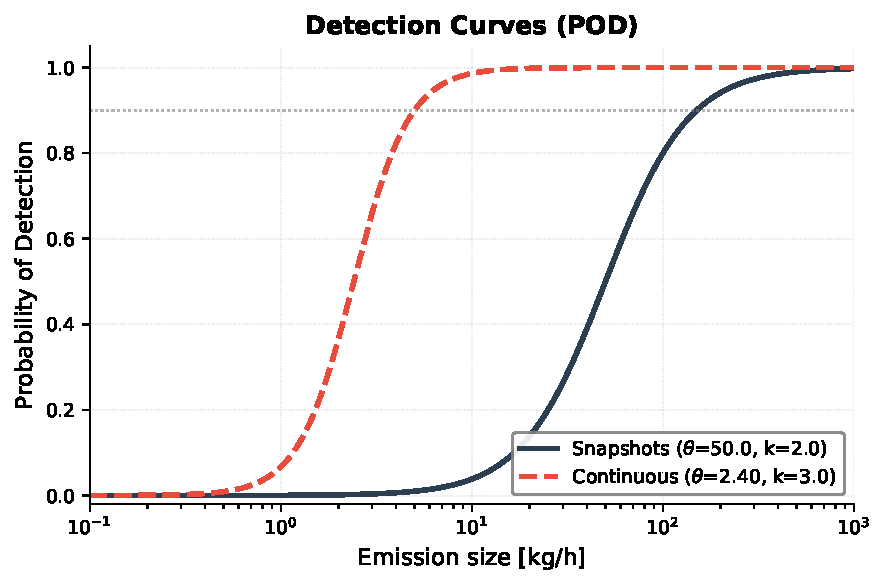
\includegraphics[width=0.8\textwidth]{figures/figure_pod_curves.pdf}
\caption{Probability-of-detection (POD) curves for the two monitoring technologies used in the baseline simulation. The snapshot sensor (solid, $\theta = 50$~kg/h, $k = 2$) represents aerial or satellite measurements with high detection thresholds. The continuous sensor (dashed, $\theta = 2.4$~kg/h, $k = 3$) represents ground-based monitoring with much lower thresholds but steeper transition. The large separation between the two curves is the key feature of the dual-technology design: continuous monitors detect small emissions that snapshot sensors miss entirely, while both technologies are reliable for large emissions.}
\label{fig:pod_curves}
\end{figure}

\subsection{Emission size distribution}

Figure~\ref{fig:size_dist} illustrates the emission size distribution and its interaction with the detection process.

\begin{figure}[h]
\centering
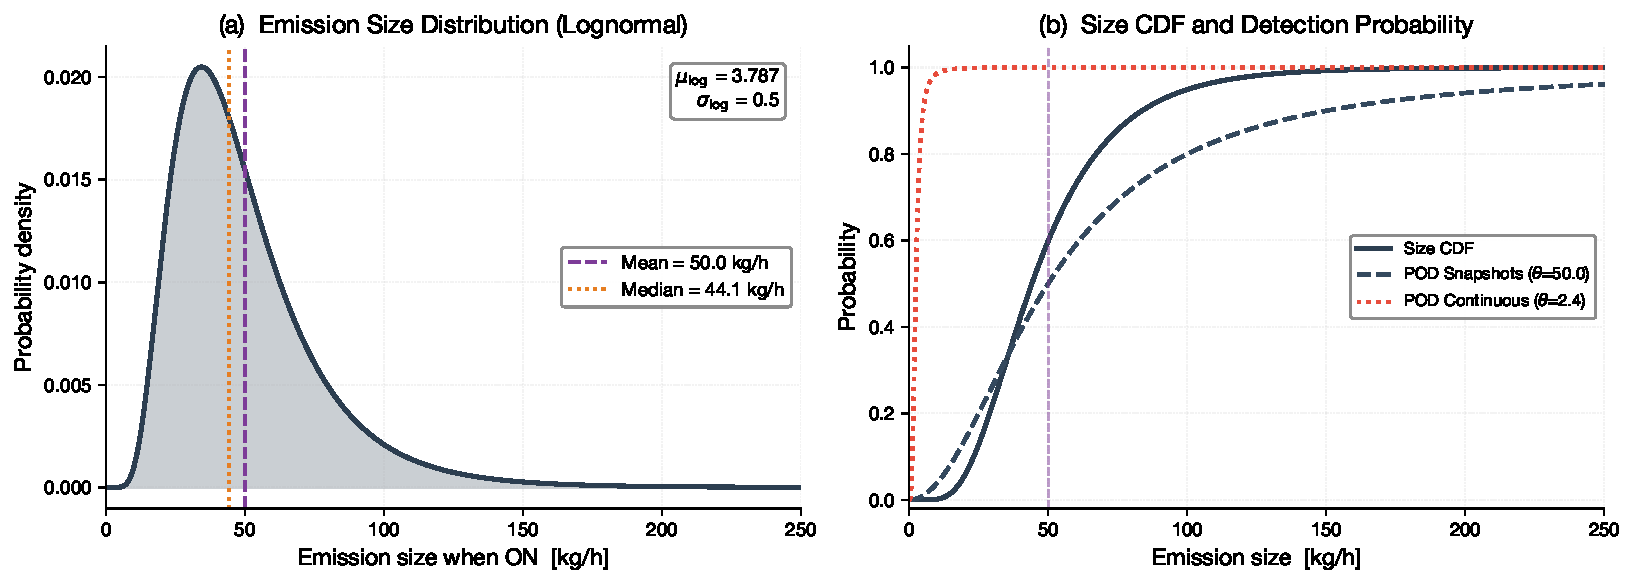
\includegraphics[width=\textwidth]{figures/figure_size_distribution.pdf}
\caption{Emission size distribution and its interaction with detection. \textbf{(a)}~The log-normal distribution of emission rates conditional on the source being active ($\mu_{\log} = 3.787$, $\sigma_{\log} = 0.5$; mean 50.0~kg/h, median 44.1~kg/h). \textbf{(b)}~Cumulative distribution of emission sizes overlaid with the POD curves of both technologies. The continuous sensor (dotted) detects nearly all emissions above 10~kg/h, while the snapshot sensor (dashed) has 50\% detection probability at 50~kg/h---close to the distribution's mean---so a substantial fraction of active emissions go undetected by snapshots alone. This illustrates why inverse-probability weighting is essential for unbiased estimation.}
\label{fig:size_dist}
\end{figure}

\subsection{Example realisations}

Figure~\ref{fig:realizations} shows three example site realisations from the baseline simulation, selected to illustrate the range of monitoring scenarios that arise under the hybrid observation model.


\begin{figure}[h]
\centering
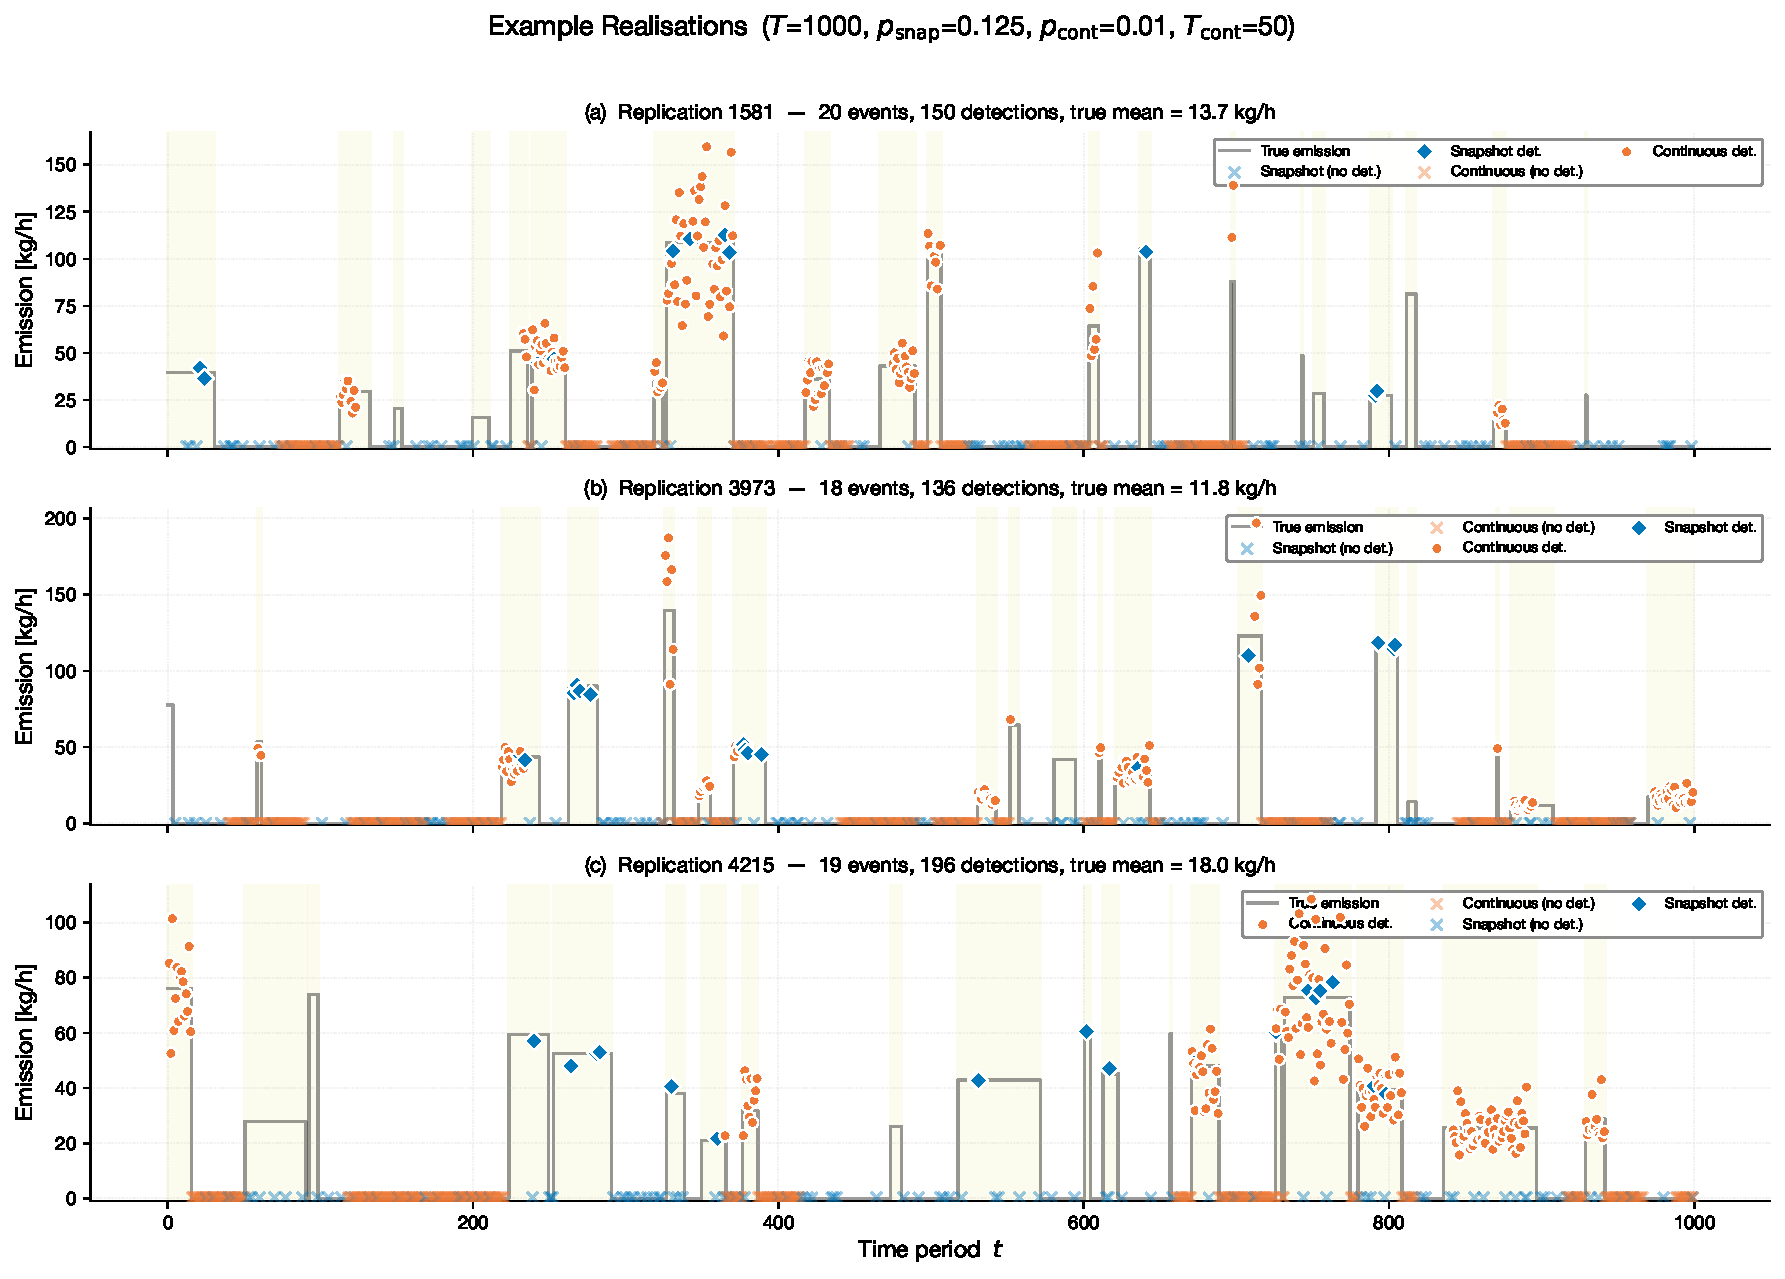
\includegraphics[width=\textwidth]{figures/figure_realizations.pdf}
\caption{Three example site realisations from the baseline simulation (\edit{$T = 1000$, $p_{\text{snap}} = 0.125$, $p_{\text{cont}} = 0.01$, $T_{\text{cont}} = 50$}). Yellow bands mark emission events (ON periods). Snapshot detections (blue diamonds) and non-detections (blue crosses) occur throughout the campaign. Continuous detections (red circles) and non-detections (red crosses) appear only during monitoring windows.
}
\label{fig:realizations}
\end{figure}

%==============================================================================
% [PB — new SI section: very-sparse cadence bias/variance comparison]
\section{Performance under Very-Sparse Snapshot Cadence}
\label{sec:sparse_SI}
%==============================================================================

\new{This section evaluates the four estimators in the limiting regime
relevant to sub-monthly survey frequencies, in which only a handful of
snapshot observations are available per facility-campaign. We set
$p_{\text{snap}} = 0.0015$ (one snapshot every 667 hours in expectation, or
approximately 1.5 snapshot observations over a 1000-hour campaign),
$p_{\text{cont}} = 0.015$ (about eight 50-hour continuous-monitoring windows
per campaign in expectation), $T_{\text{cont}} = 50$~hours, and a continuous
50\% detection threshold $\theta_c = 15$~kg/h. The continuous threshold is
deliberately set well above the baseline value so that continuous monitoring
is itself imperfect; if it were near-perfect, no estimator could improve on
the POD-weighted baseline because there would be no detection bias to
correct. The likelihood nudge factor is set to $\text{nudge} = 1.00$
(the snapshot data are too sparse to incur the discretisation-induced
upward bias in $\hat p_{\text{off}}$ that motivates the small nudge at
baseline cadence). All other parameters are at their baseline values
(Table~\ref{tab:params}). The experiment uses the same nested design as
the baseline analysis ($n_{\text{outer}} = 25$ batches of
$n_{\text{inner}} = 500$ replicates, $12{,}500$ replicates in total).}

\begin{figure}[h]
\centering
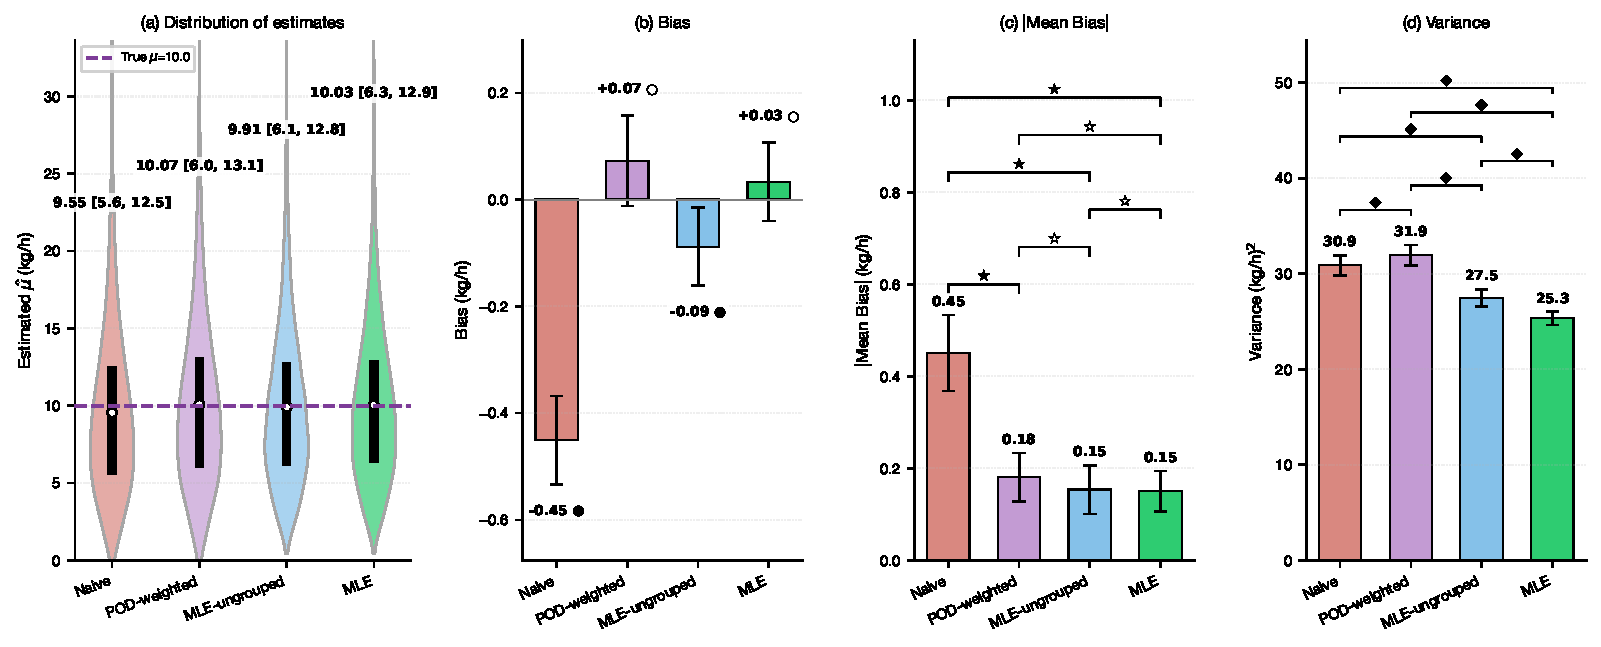
\includegraphics[width=\textwidth]{figures/figure_baseline_violin_v2_wide_sparse.pdf}
\caption{\new{Sampling distributions of the four $\hat\mu$ estimators in the
very-sparse regime ($p_{\text{snap}} = 0.0015$, $p_{\text{cont}} = 0.015$,
$T_{\text{cont}} = 50$, $\theta_c = 15$~kg/h, $T = 1{,}000$). Violin plots
show the distribution of point estimates over $12{,}500$ replicates
($25 \times 500$); the dashed horizontal line marks the true value
$\mu_{\text{true}} = 10.0$~kg/h. The MLE concentrates around the truth
with the lowest variance among the unbiased estimators; the naive
estimator is visibly biased downward.}}
\label{fig:sparse_violin}
\end{figure}

\new{Figure~\ref{fig:sparse_violin} and Table~\ref{tab:sparse_comparison}
summarise the results. The POD-weighted estimator and the MLE are both
unbiased ($t = +1.68$, $p = 0.11$ and $t = +0.86$, $p = 0.40$
respectively, n.s.), while the naive estimator is significantly biased
downward ($t = -10.67$, $p < 0.001$). The variance ordering is the same
as at baseline cadence (Naive~$<$~POD~$>$~MLE-ungrouped~$>$~MLE), and
every pairwise variance difference is statistically significant in the
expected direction ($p < 0.001$ in all cases). Quantitatively, the MLE
achieves a $20.7\%$ reduction in variance relative to the POD-weighted
estimator ($25.36$ vs.~$31.99$, paired $t = +13.18$, $p < 0.001$) and a
$7.8\%$ reduction relative to the MLE-ungrouped variant ($25.36$ vs.~$27.52$,
paired $t = +6.75$, $p < 0.001$). The latter quantifies the contribution
of the HMM-based event grouping in this regime: even when only $\sim$1.5
snapshot observations are available per facility-campaign, exploiting
the temporal correlation across the continuous-monitoring windows
yields a statistically significant variance improvement.}

\begin{table}[h]
\centering
\caption{\new{Bias, variance, and pairwise statistical tests under
very-sparse snapshot cadence ($p_{\text{snap}} = 0.0015$,
$p_{\text{cont}} = 0.015$, $T_{\text{cont}} = 50$, $\theta_c = 15$~kg/h,
$T = 1{,}000$, $n_{\text{outer}} = 25 \times n_{\text{inner}} = 500$).
Bias is reported as $\hat\mu - \mu_{\text{true}}$ with
$\mu_{\text{true}} = 10.0$~kg/h. Confidence intervals are 95\% across
the 25 outer batches. Significance markers: $^{***}\!p<0.001$,
$^{**}\!p<0.01$, $^{*}\!p<0.05$, n.s.\ otherwise.}}
\label{tab:sparse_comparison}
\begin{tabular}{lrrrr}
\toprule
Estimator         & Bias              & 95\% CI    & Variance        & RMSE \\
\midrule
Naive             & $-0.451^{***}$    & $\pm 0.083$ & $30.93$         & $5.58$ \\
POD-weighted      & $+0.073$ (n.s.)   & $\pm 0.085$ & $31.99$         & $5.66$ \\
MLE-ungrouped     & $-0.089^{*}$      & $\pm 0.072$ & $27.52$         & $5.25$ \\
\textbf{MLE}      & $+0.032$ (n.s.)   & $\pm 0.074$ & $\mathbf{25.36}$ & $\mathbf{5.04}$ \\
\bottomrule
\end{tabular}

\vspace{0.6em}

\begin{tabular}{lrr}
\toprule
Pairwise variance test (paired $t$ on 25 outer batches) & $t$ & $p$ \\
\midrule
Naive          vs.\ POD-weighted    & $-29.71$ & $<0.001^{***}$ \\
POD-weighted   vs.\ MLE-ungrouped   & $+16.08$ & $<0.001^{***}$ \\
POD-weighted   vs.\ MLE             & $+13.18$ & $<0.001^{***}$ \\
MLE-ungrouped  vs.\ MLE             & $+6.75$  & $<0.001^{***}$ \\
\bottomrule
\end{tabular}
\end{table}

\new{Two practical implications follow. First, the MLE's variance advantage
established at baseline cadence persists at sub-monthly snapshot cadence
provided that the continuous-monitoring channel is itself imperfect.
Second, in this regime the dominant source of the MLE's improvement
over the POD-weighted estimator is the temporal information contained
in the continuous-monitoring windows, which the HMM is able to exploit;
the snapshot channel contributes little additional information when so
few snapshots are available per campaign. This is consistent with the
$p_{\text{cont}}$ sweep in Figure~\ref{fig:sweep_cont}a, where the
variance ratio is maximised when continuous monitoring is sparse.}


%==============================================================================
\section{Sensitivity to Campaign Length}
\label{sec:sweep_T}
%==============================================================================

We investigate how estimation performance varies with campaign length~$T$ by sweeping $T \in \{125, 250, 500, 1{,}000, 2{,}000\}$ while holding all other parameters at baseline values. 

Figure~\ref{fig:composite_T} provides a comprehensive view of parameter recovery: the top row shows relative bias~(\%) and the bottom row shows the coefficient of variation~(CV~\%) for each MLE parameter as a function of~$T$. The time-averaged emission rate~$\hat{\mu}$ (rightmost column) also includes the POD-weighted estimator for comparison. All four parameters exhibit small relative biases that are stable or decrease with~$T$, and CV narrows monotonically. The main-paper parameter histograms (Figure~4 in the main text) correspond to the baseline $T = 1{,}000$ column of this composite.

\begin{figure}[h]
\centering
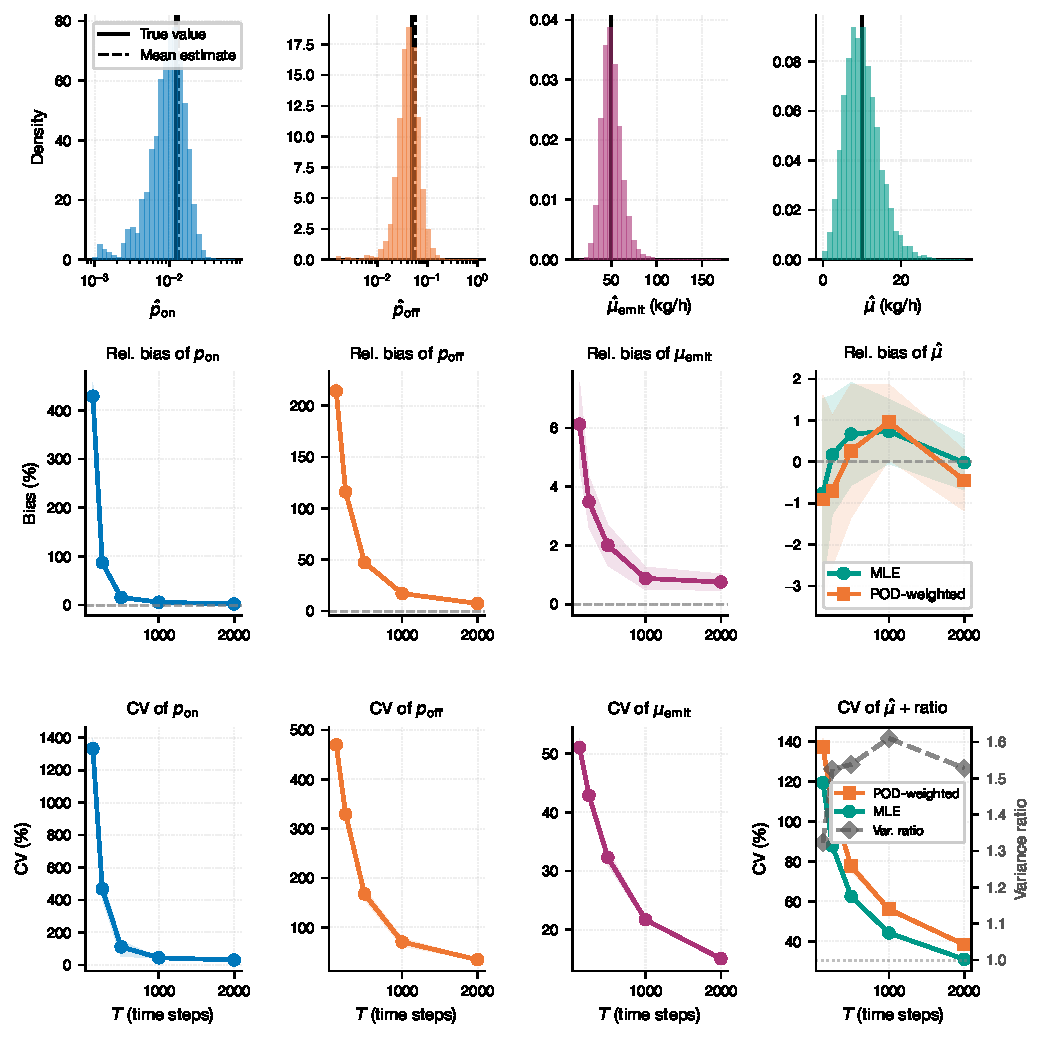
\includegraphics[width=\textwidth]{figures/figure1_composite.pdf}
\caption{Relative bias~(\%, top row) and coefficient of variation~(CV~\%, bottom row) of MLE parameter estimates as a function of campaign length~$T$. From left to right: $\hat{p}_{\text{on}}$, $\hat{p}_{\text{off}}$, $\hat{\mu}_{\text{emit}}$, and~$\hat{\mu}$ (with POD-weighted for comparison). Shaded bands show 95\% CIs. \edit{All parameters show stable or decreasing relative bias with~$T$, confirming that the small positive shifts in $(\hat p_{\text{on}}, \hat p_{\text{off}})$ reported in the main text are finite-sample effects that vanish asymptotically, consistent with the standard theory of MLEs \citep[Ch.~5]{vanderVaart1998}.} % [EVAN finite-sample-bias question]
The CV of~$\hat{\mu}_{\text{emit}}$ and~$\hat{p}_{\text{off}}$ decreases substantially with longer campaigns, reflecting the additional data available for disentangling intermittency from detection effects. The rightmost bottom panel also shows the variance ratio (red, right axis).}
\label{fig:composite_T}
\end{figure}


%==============================================================================
\section{Sensitivity to Continuous-Monitoring Parameters}
\label{sec:sweep_cont_SI}
%==============================================================================

% [PB — consolidated section: p_cont sweep (moved from main) + new T_cont sweep, presented in a single figure]
\new{This section reports two sweeps that jointly characterize the role of continuous-monitoring coverage in the MLE's variance reduction. The first sweeps the per-step probability $p_{\text{cont}}$ of triggering a continuous-monitoring window; the second sweeps the window duration $T_{\text{cont}}$. In each, all other parameters are held at baseline values. Together they decompose the expected continuous coverage fraction $T_{\text{cont}} / (T_{\text{cont}} + 1/p_{\text{cont}})$ into its two independent determinants, clarifying which aspect of continuous monitoring — frequency of window onsets or duration of each window — drives performance. Both sweeps are shown in Figure~\ref{fig:sweep_cont}.}

\begin{figure}[h]
\centering
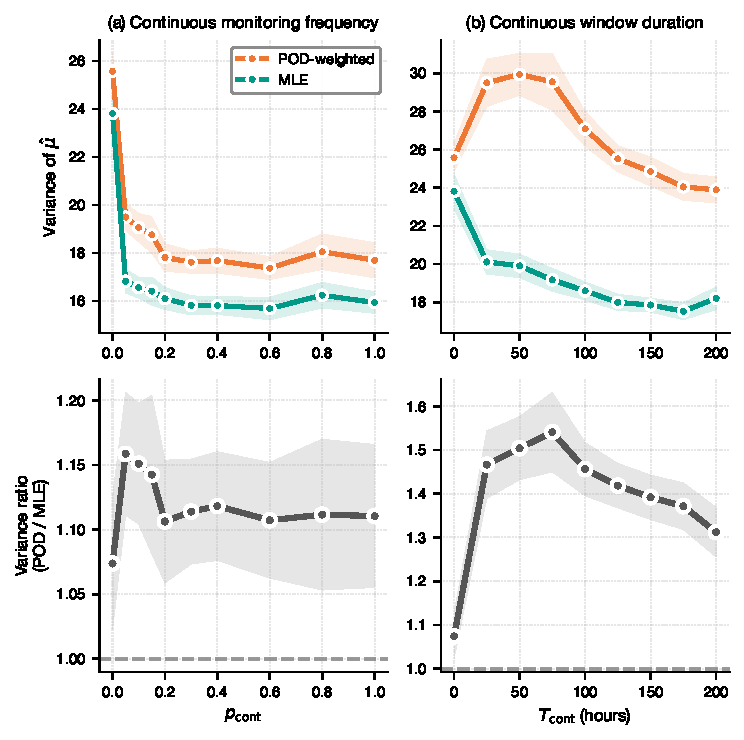
\includegraphics[width=\textwidth]{figures/figure_sweeps_cont.pdf}
\caption{\new{Sensitivity of estimation variance to the two continuous-monitoring parameters (shaded bands: 95\% CIs over 25 replicates). \textbf{(a)}~Sweep over the trigger probability $p_{\text{cont}}$, holding $T_{\text{cont}}$ at baseline. \textbf{(b)}~Sweep over the window duration $T_{\text{cont}}$, holding $p_{\text{cont}}$ at baseline. Top row: variance of the MLE and POD-weighted estimators. Bottom row: variance ratio (POD-weighted / MLE); values above the dashed line indicate lower MLE variance.}}
\label{fig:sweep_cont}
\end{figure}

\subsection{Continuous-monitoring frequency ($p_{\text{cont}}$)}
\label{sec:sweep_pcont_SI}

\new{The trigger probability $p_{\text{cont}}$ controls how often a site accumulates a window of dense temporal data. Figure~\ref{fig:sweep_cont}a shows that the MLE outperforms the POD-weighted estimator across the full range of $p_{\text{cont}}$, with the advantage markedly larger when continuous monitoring is sparse: the variance ratio peaks at approximately $1.36$ at $p_{\text{cont}} = 0$, drops to roughly $1.07$ by $p_{\text{cont}} = 0.2$, and stabilises in the $1.07$--$1.08$ range as $p_{\text{cont}}$ increases further. Two mechanisms account for this pattern. When continuous monitoring is rare, the snapshot data alone carry most of the inferential burden, and the HMM's exploitation of temporal correlation among repeated snapshots is the dominant source of variance reduction relative to the POD-weighted estimator. As continuous-monitoring coverage grows, both estimators benefit from the additional detections, and the variance gap narrows toward a regime in which most of the easy information has already been extracted by both methods.}

\subsection{Continuous-window duration ($T_{\text{cont}}$)}
\label{sec:sweep_Tcont_SI}

\new{The window duration $T_{\text{cont}}$ controls how long each continuous-monitoring window persists once triggered. Holding $p_{\text{cont}}$ at its baseline value and sweeping $T_{\text{cont}}$ varies the expected coverage fraction without changing the frequency of window onsets. Figure~\ref{fig:sweep_cont}b shows a non-monotonic pattern in the variance ratio. At $T_{\text{cont}} = 0$ (no continuous coverage), the ratio is approximately 1.35, matching the $p_{\text{cont}} = 0$ point of panel (a). As $T_{\text{cont}}$ grows, the ratio rises to a peak near 1.62 in the range $T_{\text{cont}} \in [25, 75]$ hours, then declines monotonically toward 1.34 at $T_{\text{cont}} = 200$ hours.}

\new{The location of the peak is informative. With baseline mean emission duration $\tau_{\text{emit}} = 20$ hours, windows in the 25--75 hour range are long enough to span a typical emission event in its entirety while still triggering frequently enough (under fixed $p_{\text{cont}} = 0.01$) to sample many distinct events. In this regime, the HMM can tightly constrain the hidden-state sequence within each window and the MLE extracts the maximum benefit from event-level grouping. As $T_{\text{cont}}$ grows beyond a few times $\tau_{\text{emit}}$, additional within-window observations sample the same events redundantly, and the marginal informational return of further duration declines. The POD-weighted estimator's variance also decreases at long $T_{\text{cont}}$, though more slowly, and the gap between the two methods narrows.}

\new{Read jointly, the two sweeps indicate that the MLE benefits more from a moderate number of sufficiently long windows than from many short windows at the same total coverage fraction, and that the marginal value of additional continuous-monitoring effort declines once windows comfortably exceed the characteristic emission duration.}


%==============================================================================
\section{Robustness to Grid Resolution}
\label{sec:robustness_grid}
%==============================================================================

The HMM grid search for $(p_{\text{on}}, p_{\text{off}})$ uses a geometric grid of $G$ candidate values centered on initial estimates. Since the grid resolution directly determines the precision of the search for $p_{\text{on}}$ and $p_{\text{off}}$, it is important to verify that the downstream estimates $\mu_{\text{emit}}$ and~$\hat{\mu}$ are insensitive to this choice.
In figure~\ref{fig:grid_robustness}, we vary the number of grid points $G \in \{5, 9, 15, 25, 41\}$ while keeping the geometric ratio between consecutive points fixed ($N = 500$ replications each), and confirm that the results are not sensitive to the grid resolution near the chosen resolution for other experiments ($G=15$).

\begin{figure}[h]
\centering
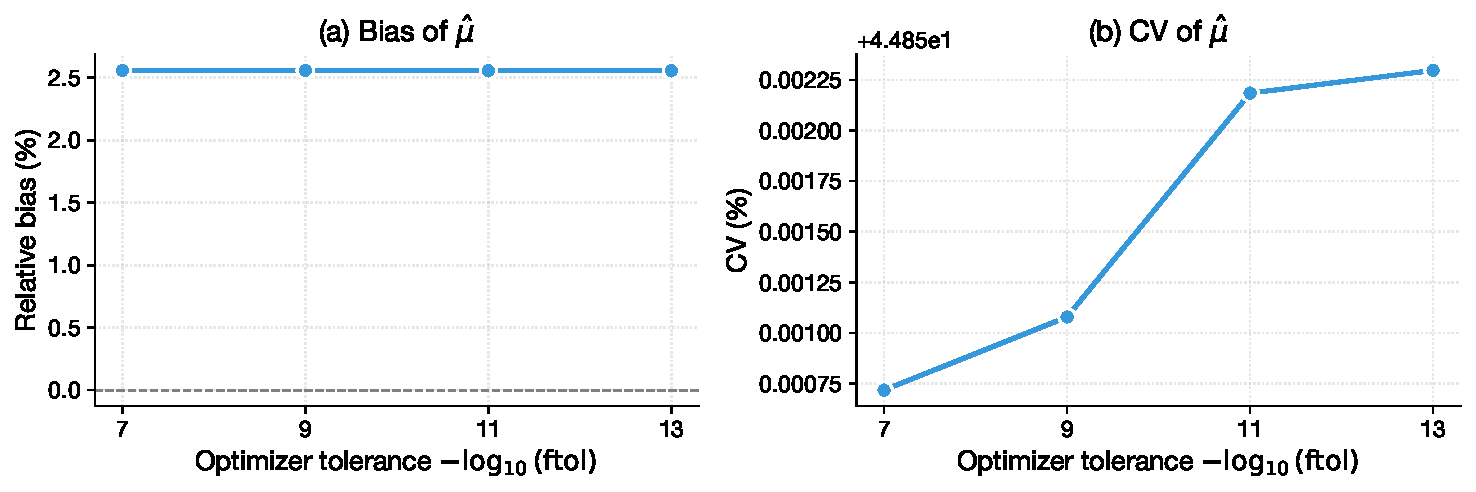
\includegraphics[width=\textwidth]{figures/figure_grid_robustness.pdf}
\caption{Robustness to HMM grid resolution. Columns show relative bias~(\%) and CV~(\%) for $p_{\text{on}}$, $p_{\text{off}}$, $\mu_{\text{emit}}$, and~$\hat{\mu}$ as a function of the number of grid points~$G$. All estimates are stable across the full range, confirming that the baseline choice ($G = 15$) is not critical.}
\label{fig:grid_robustness}
\end{figure}

%==============================================================================
\section{Sensitivity to Plume-Linking Threshold}
\label{sec:threshold}
%==============================================================================

The Bayesian posterior linking step (Step~1 of the MLE loop) classifies consecutive detections as belonging to the same emission event when the posterior probability exceeds a decision threshold~$\delta$. We use $\delta = 0.5$ as baseline (i.e., maximum-a-posteriori classification). To verify that results are not sensitive to this choice, we sweep $\delta \in \{0.2, 0.3, 0.4, 0.5, 0.6, 0.7, 0.8\}$ while holding all other parameters at baseline ($N_{\text{outer}} = 5$, $N_{\text{inner}} = 500$). Figure~\ref{fig:threshold} confirms that performance is stable across this range.

\begin{figure}[h]
\centering
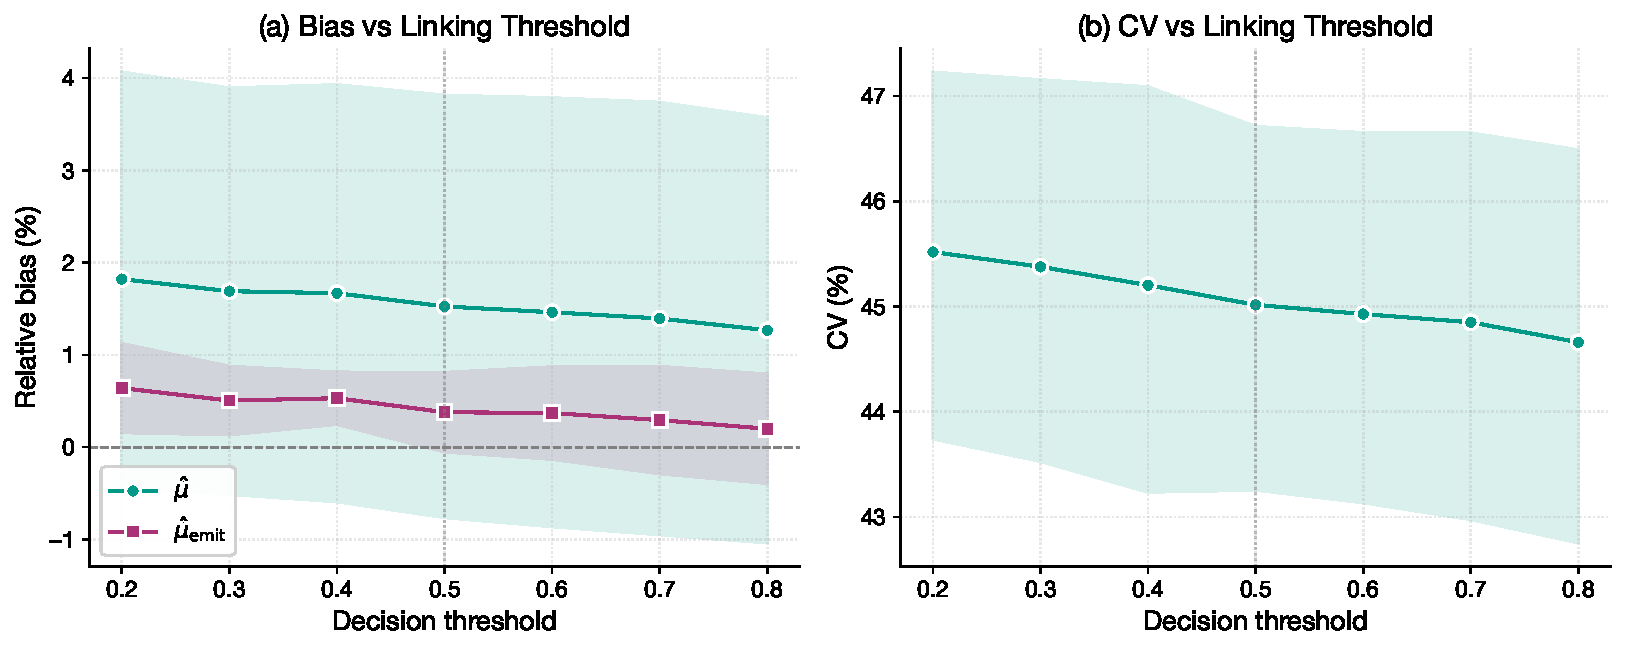
\includegraphics[width=\textwidth]{figures/figure_threshold_sweep.pdf}
\caption{Sensitivity of MLE estimates to the plume-linking decision threshold~$\delta$. \textbf{(a)}~Relative bias of~$\hat{\mu}$ and~$\hat{\mu}_{\text{emit}}$. \textbf{(b)}~Coefficient of variation of~$\hat{\mu}$. The vertical dotted line marks the baseline value $\delta = 0.5$. The true value of $\mu$ remains in the 95\% confidence interval across $\delta\in[0.2,0.8]$. The null hypothesis ``unbiased estimator'' cannot be rejected.}
\label{fig:threshold}
\end{figure}

%==============================================================================
% SI section: Sensitivity to sensor-parameter misspecification
%==============================================================================
\section{Sensitivity to Sensor-Parameter Misspecification}
\label{sec:misspec_SI}

\new{The preceding analyses assume the POD curves and noise parameters are
known exactly. In practice these are estimated from controlled-release tests
with finite sample sizes, and real-world deployment conditions may differ
from the test environment. This section characterises the sensitivity of
the estimator to this additional source of uncertainty.}

\paragraph{Choice of perturbed parameter.}
\new{The six sensor parameters $\boldsymbol{\psi} = (\theta_s, k_s, \sigma_s,
\theta_c, k_c, \sigma_c)$ enter the likelihood with very different leverage,
and a per-parameter analysis (Figure~\ref{fig:misspec_onebyone_SI}) confirms
that a single one — the snapshot $50\%$ detection threshold $\theta_s$ —
accounts for nearly all of the misspecification sensitivity at the
baseline configuration. The reasons are structural. The threshold
$\theta_s$ sets the location of the $50\%$ detection probability and
therefore directly controls the fraction of emission events the estimator
considers detectable; at baseline ($\theta_s = 50$~kg/h, lognormal
emission median $44$~kg/h) it sits in the bulk of the emission
distribution, so perturbations move a substantial share of events across
the detection boundary. The POD steepness $k_j$ governs the transition
near $\theta_j$ but not its location, and most emissions lie far from
$\theta_j$ where the POD is close to either zero or one; perturbations of
$k_j$ therefore alter the likelihood weakly. The noise parameters
$\sigma_j$ affect quantification rather than detection, and within-plume
averaging across many detections attenuates their downstream effect on
$\hat\mu$. The continuous-monitor parameters $(\theta_c, k_c, \sigma_c)$
contribute negligibly because $\theta_c = 2.4$~kg/h sits well below the
bulk of active emissions, so virtually every active event is detected
during a continuous window irrespective of small displacements of
$\theta_c$. We therefore restrict the main analysis to $\theta_s$.}

\paragraph{Experimental design.}
\new{We perturb $\theta_s$ on the log scale,
\begin{equation}
    \log \tilde\theta_s \;\sim\; \mathcal{N}(\log \theta_s^{\text{true}},\, \eta^2),
\end{equation}
where $\eta$ is a dimensionless misspecification magnitude
(approximately the relative SD of $\tilde\theta_s$ for small $\eta$). The
log-normal form keeps $\tilde\theta_s$ strictly positive and makes the
perturbation scale-invariant; the other five sensor parameters are held
at their true values. At each outer replicate we (i) draw a fresh
$\tilde\theta_s$, (ii) simulate data under $\theta_s^{\text{true}}$, and
(iii) run the MLE using $\tilde\theta_s$. This separates the data-generating
truth from the parameters used in estimation, mimicking real deployment in
which the analyst plugs in calibration estimates rather than the unknown
truth. We sweep $\eta \in \{0, 0.05, 0.1, 0.15, 0.2, 0.3, 0.5, 0.6, 0.7, 0.8\}$
with $25$ outer replicates and $500$ inner data replicates per outer
batch. Because random misspecification produces both random shifts in
$\hat\mu$ and, asymmetrically at larger $\eta$, a small systematic shift,
we report mean squared error,
\begin{equation}
    \mathrm{MSE}(\hat\mu) \;=\; \mathbb{E}\!\bigl[(\hat\mu - \mu^{\text{true}})^2\bigr],
\end{equation}
which captures both contributions in a single metric.}

\paragraph{Results.}
\new{Figure~\ref{fig:misspec} reports MSE as a function of $\eta$. At
$\eta = 0$ (correct specification), $\mathrm{MSE} = 18.1$~kg$^2$/h$^2$,
reflecting irreducible sampling variance alone. As $\eta$ grows, MSE
rises gradually: it remains within $6\%$ of its $\eta=0$ value up to
$\eta = 0.3$ (a $\sim\!30\%$ relative misspecification of $\theta_s$),
and reaches $22.2$~kg$^2$/h$^2$ at $\eta = 0.5$. Even at $\eta = 0.8$ —
corresponding to a log-normal SD of $0.8$ on $\theta_s$, far beyond the
level achievable by any reasonable controlled-release calibration — the
MLE retains an MSE advantage over the POD-weighted baseline
($28.8$ versus $29.9$~kg$^2$/h$^2$). No crossover at which the MLE loses
its advantage occurs within the range we tested. Bias remains small
throughout (less than $6\%$ of MSE at $\eta = 0.8$, and below $1\%$ for
$\eta \le 0.5$), so the rise in MSE is dominated by the variance
component induced by drawing different $\tilde\theta_s$ across outer
replicates.}

\begin{figure}[h]
\centering
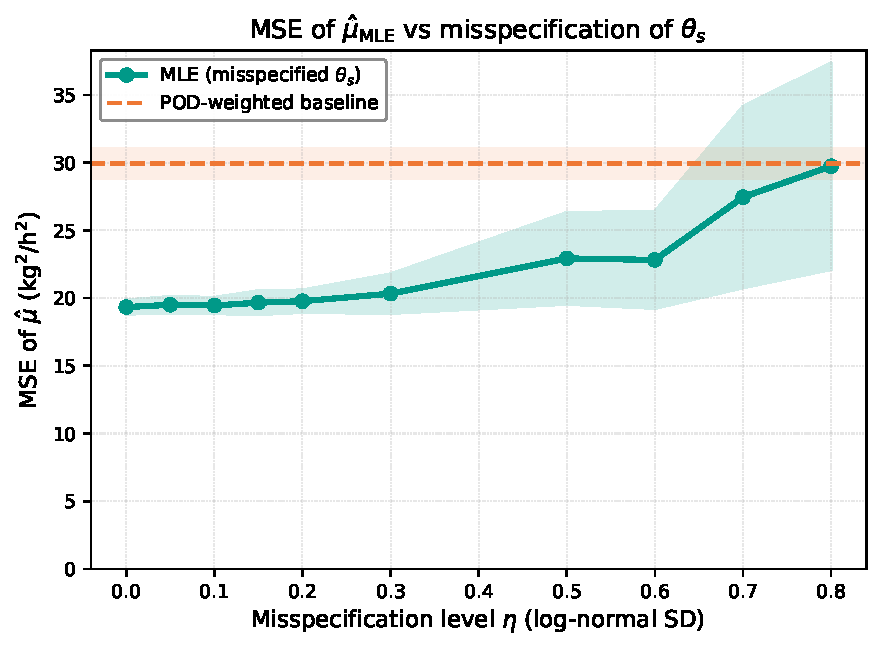
\includegraphics[width=0.85\textwidth]{figures/figure_misspec_thetas_mse.pdf}
\caption{Robustness of MLE performance to misspecification of the
snapshot $50\%$ detection threshold $\theta_s$. At each outer replicate,
$\tilde\theta_s$ is drawn log-normally around $\theta_s^{\text{true}}$
with standard deviation $\eta$ in log-space; data are generated under
$\theta_s^{\text{true}}$, while estimation uses $\tilde\theta_s$. The
horizontal dashed line marks the POD-weighted MSE under correct
specification, used as a reference baseline. The shaded band is a
$95\%$ confidence interval across $25$ outer replicates of
$\tilde\theta_s$.}
\label{fig:misspec}
\end{figure}

\paragraph{Implications.}
\new{Two implications follow. First, the MSE advantage of the MLE is
robust to the level of $\theta_s$ uncertainty likely to be encountered
after even rudimentary controlled-release characterisation: an $80\%$
log-normal SD on $\theta_s$ — well in excess of values reported in the
controlled-release literature — does not eliminate the advantage.
Second, $\theta_s$ is the single sensor parameter to which the framework
is most sensitive (Figure~\ref{fig:misspec_onebyone_SI}); refinement of
the snapshot $50\%$ detection threshold therefore yields the largest
reduction in total estimator error at the margin. Application of the
framework to a new sensor should accordingly prioritise controlled-release
coverage near the sensor's snapshot detection threshold.}


%==============================================================================
% New SI section: How to apply the framework in practice
%==============================================================================
\section{How to Apply the Framework in Practice}
\label{sec:howto_SI}

\new{This section translates the estimation procedure of Section~2 of the main text into a workflow for application to monitoring data.}

\subsection{Inputs}
\new{For each technology $j$ deployed at the facility of interest, three inputs are needed: a probability-of-detection (POD) curve, a measurement-noise parameter, and a sampling log.}

\new{The POD curve $q_j(e)$ specifies the probability that the sensor detects an emission of size $e$. The logistic form of equation~(2) of the main text is recommended, parameterized by the 50\%-detection threshold $\theta_j$ and steepness $k_j$; both are reported in published controlled-release studies for most commercial methane sensors. When only a threshold is reported, $k_j = 2$ provides a reasonable default. When multiple thresholds are reported across environmental conditions, the operational mean may be used, with uncertainty propagated via the misspecification analysis of Section~\ref{sec:misspec_SI}.}

\new{The measurement-noise parameter $\sigma_j$ is the log-scale standard deviation of quantified emission rates relative to truth in controlled-release tests. Values in the range $0.05$--$0.3$ cover most published technologies. For fenceline monitors exhibiting left-censored error distributions, the lognormal specification should be replaced by a censored variant (see the Discussion in the main text).}

\new{The sampling log is a list of four-tuples $(t_i, j_i, Y_i, D_i)$ recording the time of observation, the technology used, the detection indicator, and the measured emission rate (zero or missing for non-detections). Non-detections — time steps at which a technology was active but did not register a detection — are informative and must be recorded; their omission biases the estimator toward large values.}

\subsection{Workflow}
\new{The sampling log is first converted into the format described in Section~2 of the main text. Time steps during which no technology was active appear as gaps and are handled automatically by the multi-step transition matrix of Section~\ref{sec:multistep}. The initial value $\hat p_{\text{off}}^{(0)}$ is set from the empirical mean gap between consecutive detections; the estimator is insensitive to this choice, and a gap of a few time steps is adequate. Steps~1--3 of the main-text algorithm are then iterated until successive estimates of $(p_{\text{on}}, p_{\text{off}})$ differ by less than $10^{-3}$, which typically requires 5--15 iterations.}

\new{In our simulation studies, estimator variance is characterized through Monte Carlo replication. For application to real monitoring data, a block bootstrap that resamples at the plume level rather than the individual-observation level preserves the within-event correlation structure and provides a natural route to within-campaign confidence intervals.}

\subsection{Practical considerations}
\new{Several issues arise when applying the framework to real monitoring records. The HMM likelihood can become flat in $p_{\text{on}}$ when a facility produces fewer than roughly five detected events over the campaign; in such cases the estimate is unstable, and remedies include extending the campaign, pooling across similar facilities, or using the POD-weighted estimator instead. Continuous monitors typically have visibility windows governed by wind direction (main text, Section~2), so the sampling log should reflect visibility rather than instrument uptime — a sensor operating with no plume in its field of view contributes no information. Published POD curves are valid under the conditions in which they were measured; deployment under substantially different conditions (offshore, at night, or in high winds) calls for re-estimation of the curve or wider misspecification analysis. Finally, the MLE output $\hat\mu$ is already a time-average and should not be multiplied by a separately estimated persistence fraction.}

\subsection{What to report}
\new{For each facility, the recommended quantities to report are the point estimate $\hat\mu$ in kg/h, the estimated activity fraction $\hat\pi_{\text{on}}$ and mean event duration $1/\hat p_{\text{off}}$, the number of detected events and total observation time, and any assumed deviations from published sensor parameters together with sensitivity to these deviations as characterized in Section~\ref{sec:misspec_SI}. Reporting the latter supports future meta-analyses and enables downstream propagation of misspecification uncertainty.}


%==============================================================================
\bibliographystyle{plainnat}
\bibliography{references}

\end{document}